\documentclass{ximera}
%\usepackage{sagetex}
%% handout
%% space
%% newpage
%% numbers
%% nooutcomes

%%% You can put user macros here
%% However, you cannot make new environments

\graphicspath{{./}{module1Activity/}{module2Activity/}{module3Activity/}}

\usepackage{sagetex}
\usepackage{tikz}
\usepackage{hyperref}
\usepackage{tkz-euclide}
\usetkzobj{all}
\pgfplotsset{compat=1.7} % prevents compile error.

\tikzstyle geometryDiagrams=[ultra thick,color=blue!50!black]
 %% we can turn off input when making a master document

\outcome{Understand the different sets of numbers along with the properties of these sets.}
\author{Darryl Chamberlain Jr.}
 
\title{Subgroups of Real Numbers}

\begin{document}
\begin{abstract}
Identify the subgroup of Real numbers a number belongs to. 
\end{abstract}
\maketitle

\href{https://cnx.org/contents/mwjClAV_@8.1:0KhpF2RH@23/Real-Numbers-Algebra-Essentials}{Link to section in online textbook}

%%%%%%%%%%%%%%%%%%%%%
%%%  Objective 1  %%%
%%%%%%%%%%%%%%%%%%%%%
First, watch \href{https://mediasite.video.ufl.edu/Mediasite/Play/67aa041fe31847d7be8047e131f256b71d}{this video} to review the different sets of Real numbers. 

After watching the video, write down definitions for the following subgroups of the Real numbers. You should include examples for each (you may even want to take a sneak peak at the problems and use some of these as examples!) and descriptions of how to tell what the smallest set the number belongs to. 

\begin{itemize}
\item Natural: 
\item Whole:
\item Integers:
\item Rational:
\item Irrational:
\end{itemize}

\begin{question}

It also helps to visualize the groups in a chart. An empty chart is provided below. Fill in the subgroups and try to classify the following numbers: 

$$ -\frac{21}{7}, -\frac{7}{21}, \frac{21}{7}, \frac{\pi}{4}, \frac{4}{\pi}, \frac{0}{\pi}, \frac{\pi}{0}, \sqrt{4}, \sqrt{-4}, \sqrt{21}, \sqrt{-21} $$

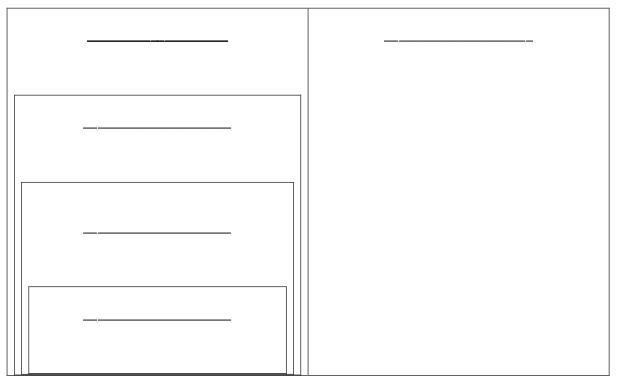
\includegraphics{realNumbersChart.png}

\textbf{\textit{Smallest subgroup the number belongs to:}}

Natural: $\answer{\frac{21}{7}}$, $\answer{\sqrt{4}}$

Whole: $\answer{\frac{0}{\pi}}$

Integer: $\answer{-\frac{21}{7}}$

Rational: $\answer{-\frac{7}{21}}$

Irrational: $\answer{\frac{\pi}{4}}$, $\answer{\frac{4}{\pi}}$, $\answer{\sqrt{21}}$

Not a Real Number: $\answer{\frac{\pi}{0}}$, $\answer{\sqrt{-4}}$, $\answer{\sqrt{-21}}$

\end{question}

\textbf{Remember to reduce first, then decide the smallest subgroup the number belongs to!}

\begin{sagesilent}
# THIS code generates a random Real Number. Options:
# Natural
# Whole
# Integer
# Rational
# Irrational
# Not a Real number
# Complex
# Dividing by zero

def generateNatural():
    denominator = ZZ.random_element(15)+1
    numerator = denominator*(ZZ.random_element(15)+1)
    negOrNo = ""
    displayProblem = [numerator**2, denominator**2, negOrNo]
    return displayProblem

def generateWhole():
    denomBefore = ZZ.random_element(15)+1
    numerator = 0
    negOrNo = ""
    maybeComplexDisplayed = sample(["Complex", "Nah"], 1)
    if maybeComplexDisplayed == "Complex":
        denominator = latex(denomBefore*pi)
    else:
        denominator = denomBefore
    displayProblem = [numerator**2, denominator**2, negOrNo]
    return displayProblem

def generateInteger():
    denominator = ZZ.random_element(15)+1
    numerator = denominator*(ZZ.random_element(15)+1)
    negOrNo = "-"
    displayProblem = [numerator**2, denominator**2, negOrNo]
    return displayProblem

def generateRational():
    numeratorBefore = ZZ.random_element(15)+7
    denominatorBefore = ZZ.random_element(15)+7
    negative = ZZ.random_element(2)
    if negative == 0:
        negOrNo = ""
    else:
        negOrNo = "-"
    counter = 0
    while gcd(numeratorBefore, denominatorBefore) >= min(numeratorBefore, denominatorBefore):
        numerator = ZZ.random_element(15)+7
        denominator = ZZ.random_element(15)+7
        counter = counter + 1
        print "Numerator: %d, \n Denominator: %d, \n Counter: %d" %(numerator, denominator, counter)
    numerator = numeratorBefore**2
    denominator = denominatorBefore**2
    displayProblem = [numerator, denominator, negOrNo]
    return displayProblem

def generateIrrational():
    numeratorBefore = ZZ.random_element(15)+1
    denominatorBefore = ZZ.random_element(15)+1
    negative = ZZ.random_element(2)
    if negative == 0:
        negOrNo = ""
    else:
        negOrNo = "-"
    integerType = type(sqrt(4))
    while type(sqrt(numeratorBefore/denominatorBefore)) == integerType:
        numeratorBefore = ZZ.random_element(15)+1
        denominatorBefore = ZZ.random_element(15)+1
    numerator = numeratorBefore
    denominator = denominatorBefore
    displayProblem = [numerator, denominator, negOrNo]
    return displayProblem

def generateNotReal():
    numeratorBefore = ZZ.random_element(15)+1
    denominatorBefore = ZZ.random_element(15)+1
    negative = ZZ.random_element(2)
    if negative == 0:
        negOrNo = ""
    else:
        negOrNo = "-"
    complexOrNotNumber = sample(["ComplexTop", "ComplexBottom", "NotNumber"], 1)[0]
    if complexOrNotNumber=="ComplexTop":
        numerator = -numeratorBefore*pi
        denominator = denominatorBefore
    elif complexOrNotNumber=="ComplexBottom":
        numerator = -numeratorBefore
        denominator = denominatorBefore*pi
    elif complexOrNotNumber=="NotNumber":
        topOrBottom = ZZ.random_element(2)
        if topOrBottom==0:
            numerator = -numeratorBefore
            denominator = 0
        else:
            numerator = -numeratorBefore * pi
            denominator = 0
    else:
        displayProblem = "Something went wrong generating a non-Real number."
        print displayProblem
    displayProblem = [numerator, denominator, negOrNo]
    return displayProblem

def generateDisplay(answer):
    if answer == "Natural":
        numerator, denominator, negOrNo = generateNatural()
    elif answer == "Whole":
        numerator, denominator, negOrNo = generateWhole()
    elif answer == "Integer":
        numerator, denominator, negOrNo = generateInteger()
    elif answer == "Rational":
        numerator, denominator, negOrNo = generateRational()
    elif answer == "Irrational":
        numerator, denominator, negOrNo = generateIrrational()
    elif answer == "NotRealNumber":
        numerator, denominator, negOrNo = generateNotReal()
    else:
        numerator, denominator, negOrNo = [0, 0, 0]
        print "\n\n\n Something went wrong choosing how to display the problem. \n\n\n\n"
    return [numerator, denominator, negOrNo]

def assignSetValue(set):
    if set == "Natural":
        value = 0
    elif set == "Whole":
        value = 1 
    elif set == "Integer":
        value = 2
    elif set == "Rational":
        value = 3
    elif set == "Irrational":
        value = 4
    elif set == "NotRealNumber":
        value = 5
    else:
        value = 6
        print "Something went wrong when assigning the set a value. Please look into this."
    return value

############ END OF DEFINITIONS ###############

listOptions=["Natural", "Whole", "Integer", "Rational", "Irrational", "NotRealNumber"]

###### QUESTION 1 #########
set1 = sample(listOptions, 1)[0]
print set1
answer1 = assignSetValue(set1)
numerator1, denominator1, negOrNo1 = generateDisplay(set1)

###### QUESTION 2 #########
set2 = sample(listOptions, 1)[0]
answer2 = assignSetValue(set2)
numerator2, denominator2, negOrNo2 = generateDisplay(set2)

###### QUESTION 3 #########
set3 = sample(listOptions, 1)[0]
answer3 = assignSetValue(set3)
numerator3, denominator3, negOrNo3 = generateDisplay(set3)

\end{sagesilent}

\textbf{Note: This part of the homework will change each time you click ``Another". You can keep clicking ``Another" to practice seeing these more difficult numbers to classify.}

\begin{question}
Which of the following is the \textbf{smallest} set of Real numbers that $\sage{negOrNo1} \sqrt{ \frac{\sage{numerator1}}{\sage{denominator1}}} $ belongs to? 

\textit{To work around current Xronos issues, input the corresponding number for the correct set. \\
Natural - 0 \\
Whole - 1 \\
Integer - 2 \\
Rational - 3 \\
Irrational - 4 \\
Not a Real Number - 5
}

$\answer{\sage{answer1}}$
\end{question}

\begin{question}
Which of the following is the \textbf{smallest} set of Real numbers that $\sage{negOrNo2} \sqrt{\frac{\sage{numerator2}}{\sage{denominator2}}} $ belongs to? 

\textit{To work around current Xronos issues, input the corresponding number for the correct set. \\
Natural - 0 \\
Whole - 1 \\
Integer - 2 \\
Rational - 3 \\
Irrational - 4 \\
Not a Real Number - 5
}

$\answer{\sage{answer2}}$
\end{question}

\begin{question}
Which of the following is the \textbf{smallest} set of Real numbers that $\sage{negOrNo3} \sqrt{\frac{\sage{numerator3}}{\sage{denominator3}}} $ belongs to? 
	
\textit{To work around current Xronos issues, input the corresponding number for the correct set. \\
Natural - 0 \\
Whole - 1 \\
Integer - 2 \\
Rational - 3 \\
Irrational - 4 \\
Not a Real Number - 5
}
	
$\answer{\sage{answer3}}$
\end{question}

\end{document}
